\documentclass[10pt]{article}
\usepackage{amsmath,amssymb}
\setlength{\oddsidemargin}{0in}
\setlength{\evensidemargin}{0in}
\setlength{\textheight}{9in}
\setlength{\textwidth}{6.5in}
\setlength{\topmargin}{-0.5in}
\usepackage{enumitem}
\usepackage{graphicx}
\usepackage{float}
\DeclareMathOperator*{\argmax}{arg\,max}
\DeclareMathOperator*{\argmin}{arg\,min}
\title{\bf Math 170S\@: Homework 7}
\date{11/21/2023}
\author{\bf Owen Jones}

\begin{document}
\maketitle
\begin{enumerate}[label=\textbf{Problem \arabic*.}]
    \item \begin{enumerate}[label=\text{\arabic*.}]
        \item $K(\mu)=P(\overline{X}\in C|\mu)$. 
        $X\sim\mathcal{N}(\mu,8100)\Rightarrow \overline{X}\sim\mathcal{N}(\mu,225)$. 
        Let $Z:=\frac{\overline{X}-\mu}{15}\sim \mathcal{N}(0,1)$.
        Let $z_\alpha:=\frac{510.77-\mu}{15}$
        $P(\overline{X}\in C|\mu)\Leftrightarrow P(Z\le z_\alpha)=\phi(\frac{510.77-\mu}{15})$.
        Thus, $K(\mu)=\phi(\frac{510.77-\mu}{15})$.
        \item $\alpha=K(530)=\phi(\frac{510.77-530}{15})=\phi(-1.282)=0.0999$
        \item $K(510.77)=\phi(\frac{510.77-510.77}{15})=\phi(0)=0.5$
        \item Graph below shows $K(\mu)$ vs. $\mu$
        \begin{figure}[H]
            \centering
            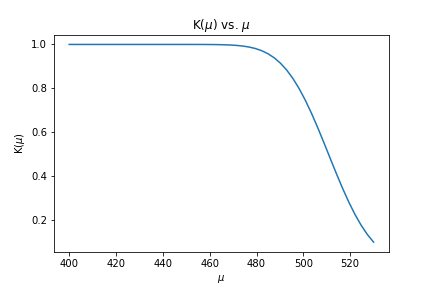
\includegraphics[scale=0.4]{Math_170_S_hw_7_q_1.png}
        \end{figure}
        \item \begin{enumerate}[label=\text{(\roman*)}]
            \item $P(\overline{X}\le 507.35)=\phi(\frac{507.35-530}{15})=0.0655$
            \item $P(\overline{X}\le 497.45)=\phi(\frac{497.45-530}{15})=0.0150$
        \end{enumerate}
    \end{enumerate}
    \item \begin{enumerate}[label=\text{\arabic*.}]
        \item By Neyman-Pearson $\forall \mu_1>0.5, \exists k$ s.t $\Lambda(x)=\frac{L(0.5)}{L(\mu_1)}\le k$ for $x\in C$ and $\Lambda(x)=\frac{L(0.5)}{L(\mu_1)}\ge k$ for $x\in C'$ where $P(\Lambda(X)\le k|H_0)=\alpha$.\\
        $\Lambda(x)=\frac{L(0.5)}{L(\mu_1)}=\frac{\displaystyle\prod_{i=1}^{10}\frac{{(0.5)}^{x_i} e^{-0.5}}{x_i!}}{\displaystyle\prod_{i=1}^{10}\frac{{(\mu_1)}^{x_i}  e^{-\mu_1}}{x_i!}}=\displaystyle\prod_{i=1}^{10}\frac{{(0.5)}^{x_i} e^{-0.5}}{{(\mu_1)}^{x_i}  e^{-\mu_1}}={(\frac{0.5}{\mu_1})}^{\displaystyle\sum_{i=1}^{10}x_i}e^{10(\mu_1-0.5)}\le k$\\
        Taking the log of both sides $\displaystyle\sum_{i=1}^{10}x_i\log(\frac{0.5}{\mu_1})+10(\mu_1-0.5)\le \log(k)$.\\
        Using the simple alternative hypothesis $H_1:\mu=\mu_1$ where $\mu_1>0.5$, it follows $\log(\frac{0.5}{\mu_1})<0$.
        Thus, $\displaystyle\sum_{i=1}^{10}x_i\ge \frac{\log(k)-10(\mu_1-0.5)}{\log(\frac{0.5}{\mu_1})}$.
        Let $c:=\frac{\log(k)-10(\mu_1-0.5)}{\log(\frac{0.5}{\mu_1})}$\\
        By Neyman-Pearson, we can define a best region $C:=\{(x_1,\ldots,x_{10}):\displaystyle\sum_{i=1}^{10}x_i\ge c\}$
        \item Want to find $c$ s.t $P(\displaystyle\sum_{i=1}^{10}x_i\ge c|H_0)=0.068$. 
        $P(\displaystyle\sum_{i=1}^{10}x_i\ge c|H_0)=1-P(\sum_{i=1}^{10}x_i<c|H_0)$, so $P(\displaystyle\sum_{i=1}^{10}x_i\ge c|H_0)=0.068\Leftrightarrow P(\sum_{i=1}^{10}x_i<c|H_0)=0.932$
        Using Python, $c=9$ gives us $P(\sum_{i=1}^{10}x_i<c|H_0)=0.932\Rightarrow P(\sum_{i=1}^{10}x_i\ge 9|H_0)=0.068$
        \item Graph below shows $K(\mu)$ vs. $\mu$
        \begin{figure}[H]
            \centering
            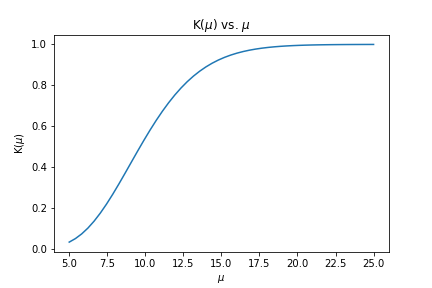
\includegraphics[scale=0.4]{Math_170_S_hw_7_q_2.png}
        \end{figure}
    \end{enumerate}
    \item \begin{enumerate}[label=\text{\arabic*.}]
        \item By Neyman-Pearson $\exists k$ s.t $\Lambda(x)=\frac{L(3)}{L(5)}\le k$ for $x\in C$ and $\Lambda(x)=\frac{L(3)}{L(5)}\ge k$ for $x\in C'$ where $P(\Lambda(X)\le k|H_0)=\alpha$.\\
        $\Lambda(x)=\frac{L(3)}{L(5)}=\frac{\displaystyle\prod_{i=1}^{n}{(\frac{1}{3})}e^{-\frac{x_i}{3}}}{\displaystyle\prod_{i=1}^{n}{(\frac{1}{5})}e^{-\frac{x_i}{5}}}=\frac{{(\frac{1}{3})}^n e^{-\frac{n\overline{x}}{3}}}{{(\frac{1}{5})}^n e^{-\frac{n\overline{x}}{5}}}={(\frac{5}{3})}^n e^{n\overline{x}(\frac{1}{5}-\frac{1}{3})}\le k$\\
        Taking the log of both sides and solving for $\displaystyle\sum_{i=1}^{n}x_i$, we obtain $\displaystyle\sum_{i=1}^{n}x_i\ge \frac{\log(k)-n\log(\frac{5}{3})}{\frac{1}{5}-\frac{1}{3}}$.
        Let $c:=\frac{\log(k)-n\log(\frac{5}{3})}{\frac{1}{5}-\frac{1}{3}}$.\\
        By Neyman-Pearson, we can define a best region $C:=\{(x_1,\ldots,x_{n}):\displaystyle\sum_{i=1}^{n}x_i\ge c\}$
        \item $P(\displaystyle\sum_{i=1}^{12}x_i\ge c)=0.1\Leftrightarrow 1-P(\displaystyle\sum_{i=1}^{12}x_i<c)=0.9$. 
        Using Python and $2\theta\displaystyle\sum_{i=1}^{12}x_i\sim \chi^2(24)$, $c=5.533$ gives us $P(\displaystyle\sum_{i=1}^{12}x_i\ge c)=P(\chi^2(24)\ge6\cdot 5.533)=0.1\Rightarrow C:=\{(x_1,\ldots,x_{n}):\displaystyle\sum_{i=1}^{n}x_i\ge 5.533\}$
        \item We choose the same critical region $C:=\{(x_1,\ldots,x_{n}):\displaystyle\sum_{i=1}^{n}x_i\ge 5.533\}$.
    \end{enumerate}  
    \item \begin{enumerate}[label=\text{\arabic*.}]
        \item $\lambda=\frac{L(\hat{\omega})}{L(\hat{\Omega})}=\frac{L(230)}{L(\overline{x})}=\frac{\displaystyle \prod_{i=1}^{n}\frac{1}{\sqrt{20\pi}}e^{-\frac{{(x_i-230)}^2}{20}}}{\displaystyle \prod_{i=1}^{n}\frac{1}{\sqrt{20\pi}}e^{-\frac{{(x_i-\overline{x})}^2}{20}}}=\frac{e^{-\displaystyle\sum_{i=1}^{n}\frac{{(x_i-230)}^2}{20}}}{e^{-\displaystyle\sum_{i=1}^{n}\frac{{(x_i-\overline{x})}^2}{20}}}\\
        =\exp(-\frac{1}{20}(\displaystyle\sum_{i=1}^{n}{(x_i-230)}^2-{(x_i-\overline{x})}^2))=\exp(-\frac{1}{20}({(n\overline{x}^2-460n\overline{x}+n{230}^2)}))\\
        =\exp(-\frac{n}{20}{(\overline{x}-230)}^2)\le k\Rightarrow -\frac{n}{10}{(\overline{x}-230)}^2\le \log(k)\Rightarrow {(\overline{x}-230)}^2\ge-\frac{20}{n}\log(k)\Rightarrow \frac{|\overline{x}-230|}{\frac{10}{\sqrt{n}}}\ge\sqrt{2\log(\frac{1}{k})}=c$.
        \item Because $Z=\frac{\overline{x}-230}{\frac{10}{\sqrt{n}}}\sim \mathcal{N}(0,1)$ set $c=z_0.1=1.282$. If $\overline{x}=232.6$ and $n=16$, then we should choose to accept $H_0$.
        \item $P(Z>\frac{232.6-230}{\frac{10}{\sqrt{16}}})=1-\phi(\frac{232.6-230}{\frac{10}{\sqrt{16}}})=0.1492$
    \end{enumerate}
\end{enumerate}
\end{document}